
\chapter{Path Planning}
\label{chap:planning}


Chapter \ref{chap:pid} explored the problem of selecting a control
signal to drive a one-dimensional system into a desired goal state.
This Chapter will explore the more general problem of controlling
multi-dimensional systems in the presence of obstacles.

Broadly speaking, control algorithms can be broken into two
categories: \vocab{reactive} and \vocab{planning-based}.  In a
reactive system the control signal is determined solely by comparing
the current state of the system to the goal configuration. The PID
controller introduced in Chapter \ref{chap:pid} is an example of a reactive
controller.

In contrast, planning-based controllers explicitly search for a
sequence of steps that will move the state of the system into a goal
configuration. Planning-based control tends to be more appropriate in
constrained control problems such as navigating in the presence of
obstacles.  In these scenarios a reactive controller may drive the
system into a dead end, where a planning-based controller is able to
look ahead to avoid actions that won't lead to the goal.  This chapter
will focus on planning-based controllers.


\section{Configuration Spaces}

Robots come in all shapes and sizes, from tiny puck-shaped robots to
humanoid robots with dozens of degrees of freedom.
\vocab{Configuration Spaces} provide a common framework for expressing
the state of a robot within its environment.  A robot's configuration
$\mathbf{q}$ is a vector that contains all of the information
necessary to completely specify the location of a robot and all of its
constituent parts.  For the locomotive robot from Chapter \ref{chap:pid},
$\mathbf{q}$ would be a single scalar value indicating the robot's
location on the tracks.  For a humanoid robot, $\mathbf{q}$ would
include all of the robot's joint angles as well as the robot's
position and orientation within its workspace.  The full space of
possible configurations is referred to as the robot's
\vocab{Configuration Space} or \vocab{C-space} and is expressed as
$\mathbf{q} \in \mathcal{C}$.

While $\mathbf{q}$ may be high-dimensional, the world that the robot
inhabits, $\mathcal{W}$, has only three spatial dimensions (or two if
we are considering a planar path-planning problem). The mapping from a
configuration $\mathbf{q}$ to the region of space occupied by a robot is
denoted $\mathcal{A}(\mathbf{q}) \subset \mathcal{W}$ where
$\mathcal{W}=\mathbb{R}^3$ or $\mathcal{W}=\mathbb{R}^2$.


In most workspaces there will be configurations that are impossible
because they would place some part of the robot inside an obstacle. We
can denote the region of space occupied by obstacles as $\mathcal{O}
\subset \mathcal{W}$.  For the purposes of planning it is useful to
map these obstacles into the configuration space of the robot.  The
result is called the \vocab{C-space obstacle region}
$\mathcal{C}_{obs}$ and can be expressed as $\mathcal{C}_{obs} =
\{\mathbf{q} \in \mathcal{C} \mid \mathcal{A}(\mathbf{q}) \cap
\mathcal{O} \neq \emptyset\}$.  The unobstructed portion of of the
configuration space is denoted $\mathcal{C}_{free}$ where
$\mathcal{C}_{free} = \mathcal{C} - \mathcal{C}_{obs}$.

\begin{figure}
\begin{center}
\fbox{\includegraphics[]{planning/figs/workspace.pdf}}
\end{center}
\caption{Example of a triangular robot in a planar environment.}
\label{fig:workspace}
\end{figure}

Figure \ref{fig:workspace} provides an example of a triangular robot
in a two-dimensional workspace containing two obstacles. This robot
may translate within the workspace but may not rotate.  This example is
atypical in that both $\mathcal{W}$ and $\mathcal{C}$ are
two-dimensional.  If we allowed the robot to rotate,
$\mathbf{\mathbf{q}}$ would require an additional dimension to
represent the robot's orientation.  The resulting configuration space
would be expressed as $\mathcal{C} = \mathbb{R}^2 \times
\mathbb{S}^1$, where $\mathbb{S}$ represents the set of real-valued
numbers representing an angle or a point on a circle.  If we were to
additional appendages to the robot, like a trailer and an articulated
arm, the dimensionality of $\mathcal{C}$ would increase still more.


\begin{figure}
\begin{center}
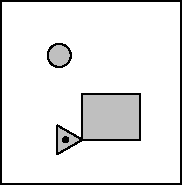
\includegraphics[]{planning/figs/pg_0001.pdf} \hspace{1em}
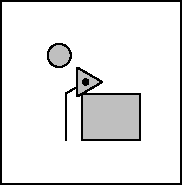
\includegraphics[]{planning/figs/pg_0003.pdf}\hspace{1em}
\includegraphics[]{planning/figs/pg_0008.pdf}

\vspace{1em}

\includegraphics[]{planning/figs/pg_0010.pdf}\hspace{1em}
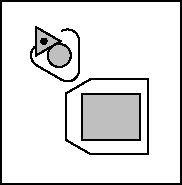
\includegraphics[]{planning/figs/pg_0014.pdf}\hspace{1em}
\includegraphics[]{planning/figs/pg_0015.pdf}
\end{center}
\caption{Determining $\mathcal{C}_{obs}$.  The bottom-right figure
  illustrates $\mathcal{C}_{obs}$ and $\mathcal{C}_{free}$ for the
  environment shown in Figure \ref{fig:workspace}.}
\label{fig:c_obs}
\end{figure}

Figure \ref{fig:c_obs} illustrates the relationship between the shape
of the robot, the locations of the obstacles and $\mathcal{C}_{obs}$.
In this case, we can imagine determining $\mathcal{C}_{obs}$ by tracking
$\mathbf{q}$ as we slide the robot around the boundaries of the two
obstacles.


The example in Figure \ref{fig:c_obs} is only intended to illustrate
the relationship between $\mathcal{A}(\mathbf{q})$ and
$\mathcal{C}_{obs}$.  It doesn't represent a general algorithm for
solving the problem. The problem of determining $\mathcal{C}_{obs}$
for arbitrary robots and obstacle shapes is not straightforward,
particularly in higher-dimensional configuration spaces.  In practice,
we don't typically attempt to calculate $\mathcal{C}_{free}$ before
searching for a plan.  It is usually more computationally efficient to
check configurations as-needed when they arise during the planning
process.

One shortcut for approximating $\mathcal{C}_{obs}$ is to represent
both obstacles and $\mathcal{A}(\mathbf{q})$ as spheres, or as sets of
spheres.  As long as the spheres are large enough to completely
enclose the objects, any non-overlapping configuration is guaranteed
to be in $\mathcal{C}_{free}$. This reduces collision detection to the
problem of calculating distances between object centers.

% Exercise?? draw circular approximation of C_free

Figure \ref{fig:arm} provides a second example of a robot and the
corresponding configuration space.  This is a planar two-link
articulated arm. For this robot $\mathcal{C} = \mathbb{S}^2$.


\begin{figure}
  \begin{center}  
    \begin{subfigure}[]{0.45\textwidth}
      \begin{center}
        \includegraphics[]{planning/figs/arm_cspace/arm_diagram.pdf}
      \end{center}
      \caption{2D robot arm with two degrees of freedom.  For this robot
        $\mathbf{q} = [\Theta_1, \Theta_2]^T$.}
    \end{subfigure} \hspace{1em}
    \begin{subfigure}[]{0.45\textwidth}
      \begin{center}  
        \includegraphics[]{planning/figs/arm_cspace/arm_world.pdf}
      \end{center}  
      \caption{An example of a possible configuration of the arm along
        with a pair of obstacles. Notice that $\mathcal{O}_2$ is close
        enough to the arm to prevent the first link one from making a
        full rotation.}
      \label{fig:arm_world}
    \end{subfigure}
    
    
    \begin{subfigure}[]{0.45\textwidth}
      \begin{center}  
        \includegraphics[]{planning/figs/arm_cspace/arm_c_space.pdf}
      \end{center}  
      \caption{An illustration of $\mathcal{C}_{obs}$ for the robot
        configuration illustrated in \ref{fig:arm_world}. The colors
        indicate configurations that intersect with the corresponding
        objects in  \ref{fig:arm_world}. }
      \label{fig:arm_c_space}
    \end{subfigure}\hspace{1em}
    \begin{subfigure}[]{0.45\textwidth}
      \begin{center}  
        \includegraphics[]{planning/figs/arm_cspace/arm_torus.pdf}
      \end{center}  
      \caption{The configuration space from \ref{fig:arm_c_space}
        represented as a torus.  The black lines are located at
        $\theta_1 = 180/-180$ and $\theta_2 = 180/-180$.  We could
        imagine creating \ref{fig:arm_c_space} by cutting along these
        lines and unwrapping the surface. }
    \end{subfigure}
    
  \end{center}
  \caption{Configuration space visualizations for a planar two-link
    robot arm.}
  \label{fig:arm}
\end{figure}





\subsubsection*{Summary of Notation}

\begin{itemize}
  \item $\mathcal{W}=\mathbb{R}^3$ (or $\mathcal{W}=\mathbb{R}^3$) -
    The workspace containing the robot
  \item $\mathbf{q}$ - The robot's configuration
  \item $\mathcal{C}$ - The robot's configuration space
  \item $\mathcal{A}(\mathbf{q}) \subset \mathcal{W}$ - The region of space
    occupied by robot $\mathcal{A}$ in configuration $\mathbf{q}$
  \item $\mathcal{O} \subset \mathcal{W}$ - The region of space
    occupied by obstacles
  \item $\mathcal{C}_{obs}$ - The subset of the configuration space
     that is unreachable because it involves the robot intersecting with an
     obstacle.
  \item $\mathcal{C}_{free}$ - The subset of the configuration space that is
    accessible to the robot
\end{itemize}


\subsection{The Path Planning Problem}



\begin{figure}
\begin{center}
  \includegraphics[]{planning/figs/path_c_obs.pdf}
  \includegraphics[]{planning/figs/path_world.pdf}
\end{center}
\caption{Left: A valid path from an initial configuration
  $\mathbf{q}_{I}$ to a goal configuration $\mathbf{q}_{G}$. Right:
  The robot trajectory corresponding to the indicated path. }
\label{fig:path_triangle}
\end{figure}

\begin{figure}
  \begin{center}

      \includegraphics[valign=t]{planning/figs/arm_cspace/arm_c_space_motion.pdf}
      \includegraphics[valign=t]{planning/figs/arm_cspace/arm_world_motion.pdf}

\end{center}
\caption{Left: A valid path from an initial configuration
  $\mathbf{q}_{I}$ to a goal configuration $\mathbf{q}_{G}$. Right:
  The robot trajectory corresponding to the indicated path. }
\label{fig:path_arm}
\end{figure}



Once $\mathcal{C}_{free}$ is determined, the path-planning problem is
conceptually simple.  All we need to do is find a continuous path in
$\mathcal{C}_{free}$ from some starting configuration $\mathbf{q}_{I}$
to the goal configuration $\mathbf{q}_{G}$.  This standard formulation
(sometimes called \vocab{the piano movers problem}) allows us to avoid
re-thinking the path planning problem for each new robot or
environment.  All of robotic path planning boils down to finding a
path from one point to another within a known subset of some
(potentially high-dimensional) space.  Figures \ref{fig:path_triangle}
and \ref{fig:path_arm} show examples of valid paths for the triangle
robot and the two-link arm respectively.


%% EXERCISES:
%% Consider the 2d triangular robot below.  C-space is $R^2$.  Draw $A(\mathbf{q})$ for
%% \mathbf{q} = (2,3), \mathbf{q}=(0,0)

%% Now consider these obstacles:
%% Draw C_{obs}

%% Cart pole $R^1 \times S^1$
%% Repeat above


\subsection{Constraints}

The discussion above assumes that any robot configuration is allowed,
as long as the robot doesn't intersect with an obstacle. In practice,
there are often additional constraints on the set of possible
configurations. These constraints can be classified as
\vocab{holonomic} or \vocab{non-holonomic}.

\subsubsection{Holonomic Constraints}

Holonomic constraints result from physical restrictions that make it
impossible for the robot to enter some regions of the configuration
space.  For example, the elbow joint on a robotic arm may only have a
90 degree range of motion.  Holonomic constraints don't significantly
complicate the path planning problem: we can simply extend our notion
of $\mathcal{C}_{free}$ to exclude restricted regions.

\subsubsection{Non-Holonomic Constraints}

Non-holonomic constraints don't directly restrict which regions of the
space are accessible. Instead, they restrict how the robot can move
from one configuration to another.  A classic example of a
non-holonomic constraint is the inability of a car to slide sideways
into a parking spot.  There is no constraint preventing the car from
being in the parking spot, but the mechanics of the vehicle prevent it
from following a straight-line path to the desired configuration.
Non-holonomic constraints can also arise from system dynamics: A
vehicle moving at 5 miles per hour can easily make a 30 degree turn,
while a vehicle moving at 50 miles per hour would roll over.
Non-holonomic constraints of this sort are referred to as
\vocab{kino-dynamic constraints}.  Non-holonomic constraints
complicate the path planning problem and require the use of
specialized algorithms.


% Thought questions....
\subsection*{Stop and Think}

\begin{exercise}
  Draw  $\mathcal{C}_{free}$ and $\mathcal{C}_{obs}$ for the world pictured below:

  \begin{center}
\fbox{\includegraphics[]{planning/figs/exercises/workspace_hw.pdf}}
\end{center}
  
  Assume that this is the same non-rotating triangular robot
  illustrated in Figures \ref{fig:workspace} and \ref{fig:c_obs}.
\end{exercise}

\begin{exercise}

  The robot in Figure \ref{fig:workspace} has a configuration space
  that can be expressed as $\mathcal{C} = \mathbb{R}^2$, the robot in
  Figure \ref{fig:arm} had a configuration space expressed as
  $\mathcal{C} = \mathbb{S}^2$.  Imagine a more complex robot that
  combines attributes of these two examples.  This new robot is a
  triangle robot that is able to translate, rotate in place, and is
  equipped with a two-link robotic arm.  How many degrees of freedom
  does this robot have?  How would we express configuration space for
  this robot?
  %(R^2 x S^3)
\end{exercise}

\begin{exercise}
Some configurations of a robotic arm may be impossible because of
self-collisions.  Is this an example of a holonomic or a
  non-holonomic constraint?
\end{exercise}

\begin{exercise}
In the text above we used set-builder notation to express the
C-obstacle region as as $\mathcal{C}_{obs} = \{\mathbf{q} \in
\mathcal{C} \mid \mathcal{A}(\mathbf{q}) \cap \mathcal{O} \neq
\emptyset\}$, where $\mathcal{O}$ represents the subset of
$\mathcal{W}$ occupied by obstacles.  What set of configurations are represented by  $\{\mathbf{q} \in
\mathcal{C} \mid ( \mathcal{A}(\mathbf{q}) \cup \mathcal{O}) \subseteq
\mathcal{O}\}$?
  \end{exercise}

\section{Planning Algorithms}

The general path planning problem outlined above is conceptually
simple but computationally difficult.  Path planning has been shown to
be PSPACE-Hard, making it extremely unlikely that we will ever have a
polynomial time algorithm that is guaranteed to find a path if one
exists.  This means that practical planning algorithms necessarily
involve compromises in completeness or involve attacking simplified
versions of the problem.  The remainder of this chapter will explore
several approaches to planning.


\section{Grid-Based Search}
\label{sec:graph_search}


\begin{figure}
\begin{center}
\includegraphics[]{planning/figs/grid1.pdf} \hspace{1em}
\includegraphics[]{planning/figs/grid2.pdf} \hspace{1em}
\includegraphics[]{planning/figs/grid3.pdf}
\end{center}
\caption{Discretizing the configuration space.  The figure on the left
  shows a uniform grid overlaying the configuration space.  In the
  center figure, all grid cells that overlap with $\mathcal{C}_{obs}$
  have been marked as inaccessible.  The figure on the right shows the
  state space graph that results if all accessible cells are connected
  to their neighbors. }
\label{fig:discretization}
\end{figure}


One way to simplify the planning problem is to perform a uniform
discretization of the configuration space and the space of possible
actions.  For example, it is common to handle holonomic 2D navigation
problems by overlaying the 2D configuration space with a grid.  Actions
are restricted to moving between four-connected or eight-connected
grid cells.  Figure \ref{fig:discretization} illustrates one possible
discretization of the triangle-robot configuration space described in
the previous section.  The result is a graph where the vertices
represent states and the edges represent actions.

Notice that the discretization in Figure \ref{fig:discretization}
makes it impossible for the robot to find a path that passes between
the two obstacles.  This highlights a trade-off between the
granularity of the discretization and the quality of the possible
solutions.  We can make our discretization arbitrarily close to the
continuous version of the problem by reducing the granularity, but
finer discretizations come at the cost of more grid cells which
increases the cost of planning.


\begin{listing}[H]
\begin{minted}[mathescape,linenos,
               fontsize=\small,
               frame=single,
               framesep=2mm]{python}

def search(problem):
    """
    Args:
        problem: a problem instance that provides three methods:

              problem.start() -       returns the start state
              problem.goal()  -       returns the goal state
              problem.successors(s) - returns the states that are 
                                      adjacent to s

    Returns:                              
        True if there exists a sequence of states leading from
        problem.start() to problem.goal(), or False if no such
        path exists
    """
    
    frontier = Collection()  # The collection of states that are
                             # currently eligible for expansion         
             
    closed = set()           # The set of states that have already
                             # been expanded

    frontier.add(problem.start())  # Initialize the search by adding
                                   # the start state to the frontier

    while not frontier.is_empty():
        cur_state = frontier.pop()  # Select the next eligible state
                                    # to expand

        closed.add(cur_state)       # Make sure that this state can't 
                                    # be added to the frontier again

        if cur_state == problem.goal():  # Success!
            return True
        
        else:
            # Add the neighbors of the selected state to the frontier...
            for next_state in problem.successors(cur_state):
                if (next_state not in closed and
                        next_state not in frontier):
                    frontier.add(next_state)
                        
    return False   # No path was found!

\end{minted}
\caption{Basic graph search algorithm.}
\label{lst:graph_search}
\end{listing}

Once a search problem has been formulated as a graph, we can use
standard graph-search algorithms to find a permissible path to the
goal.  Listing \ref{lst:graph_search} presents the basic graph search
algorithm. The algorithm works outward from the start state,
maintaining a collection of states on the frontier of the region we
have already searched.  At each iteration, we select a state from the
frontier and add its neighbors back into the frontier.  This process
continues until the goal state is selected from the frontier.

Selecting and processing a state from the frontier is referred to as
\emph{expansion}. Maintaining a \emph{closed set} allows us to avoid
re-processing states that have already been expanded.  Each time a
state is expanded it is added to the closed set.  Once a state is
closed, the check on line 39 ensures that it will never be added back
into the frontier.  This check prevents the algorithm from considering
paths containing cycles.

The collection type used to store the frontier determines the order
that the states are expanded during search.  When a queue is used, the
algorithm in Listing \ref{lst:graph_search} performs a
breadth-first-search (BFS), while the use of a stack results in
depth-first-search (DFS).

For search problems with uniform step costs, BFS is both
\vocab{complete} and \vocab{optimal}.  A complete search algorithm is
guaranteed to find a path if one exists.  An optimal search algorithm
is guaranteed to find the lowest-cost path.  BFS is optimal in the
sense that it is guaranteed to find the path with the fewest possible
steps.  By storing the frontier in a FIFO queue we ensure that all
paths of length $n$ are explored before we explore any paths of length
$n+1$.

In contrast, DFS is neither complete nor optimal. In the case of
an infinite graph, DFS could potentially perform infinite expansions
away from the goal state, even if the goal could be reached within only a
small number of steps.  The advantage of DFS is that it requires less
memory to store the frontier.  The number of nodes in the frontier
grows linearly for DFS but it may grow exponentially for BFS,
depending on the structure of the search problem.


\begin{figure}
  \begin{center}
    \begin{subfigure}[t]{0.3\textwidth}
      \includegraphics[width=1.25in]{planning/figs/bfs_0001.pdf}
       \caption{One expansion}
    \end{subfigure}
    \begin{subfigure}[t]{0.3\textwidth}
      \includegraphics[width=1.25in]{planning/figs/bfs_0002.pdf}
       \caption{Two expansions}
    \end{subfigure}
    \begin{subfigure}[t]{0.3\textwidth}
      \includegraphics[width=1.25in]{planning/figs/bfs_0009.pdf}
       \caption{Nine expansions}
    \end{subfigure}

    \vspace{.2in}

    \begin{subfigure}[t]{0.3\textwidth}
      \includegraphics[width=1.25in]{planning/figs/bfs_0081.pdf}
       \caption{81 expansions}
    \end{subfigure}
    \begin{subfigure}[t]{0.3\textwidth}
      \includegraphics[width=1.25in]{planning/figs/bfs_0350.pdf}
       \caption{350 expansions}
    \end{subfigure}
    \begin{subfigure}[t]{0.3\textwidth}
      \includegraphics[width=1.25in]{planning/figs/bfs_0641.pdf}
       \caption{641 expansion}
    \end{subfigure}

\end{center}
  \caption{BFS search example.  The cell containing the start state is
    colored green and the goal state is colored gold. States in the
    frontier are shown in blue.  States in the closed set are shown in
    gray.  The final path is shown in red. }
\label{fig:bfs}
\end{figure}




\begin{figure}
  \begin{center}
    \begin{subfigure}[t]{0.3\textwidth}
      \includegraphics[width=1.25in]{planning/figs/dfs_0001.pdf}
       \caption{One expansion}
    \end{subfigure}
    \begin{subfigure}[t]{0.3\textwidth}
      \includegraphics[width=1.25in]{planning/figs/dfs_0002.pdf}
       \caption{Two expansions}
    \end{subfigure}
    \begin{subfigure}[t]{0.3\textwidth}
      \includegraphics[width=1.25in]{planning/figs/dfs_0009.pdf}
       \caption{Nine expansions}
    \end{subfigure}

    \vspace{.2in}

    \begin{subfigure}[t]{0.3\textwidth}
      \includegraphics[width=1.25in]{planning/figs/dfs_0081.pdf}
       \caption{81 expansions}
    \end{subfigure}
    \begin{subfigure}[t]{0.3\textwidth}
      \includegraphics[width=1.25in]{planning/figs/dfs_0350.pdf}
       \caption{350 expansions}
    \end{subfigure}
    \begin{subfigure}[t]{0.3\textwidth}
      \includegraphics[width=1.25in]{planning/figs/dfs_0477.pdf}
       \caption{477 expansion}
    \end{subfigure}

\end{center}
\caption{DFS search example.}
\label{fig:dfs}
\end{figure}


Figure \ref{fig:bfs} illustrates a BFS search in our triangle-world
workspace.  Figure \ref{fig:dfs} illustrates a DFS search.


\subsection{Returning A Path}

The careful reader will notice that the algorithm in Listing
\ref{lst:graph_search} doesn't actually return a path to the goal.  It
only determines whether such a path exists.  In order to reconstruct
the path we need to maintain an auxiliary data structure that stores
backward references from each state to the state that precedes it.
Once the goal is reached, the path can be reconstructed by following
the backward references from the goal back to the start state and then
reversing the steps.  Listing \ref{lst:node_search} shows a possible
Python implementation of the necessary data type and an appropriately
updated version of the algorithm from Listing \ref{lst:graph_search}.

The containment check on line 40 of Listing \ref{lst:node_search}
requires some clarification.  The goal here is to avoid exploring
multiple paths that pass through the same state.  If the frontier
already contains a node for a state, we don't want to add another node
that represents a different route to that state.  This means that the
test on line 40 is \emph{not} checking to see if the indicated Node is
in the frontier, it is checking to see if any Node in the frontier
contains \mintinline {python}{new_state}.  Removing this check would
not impact the correctness of the algorithm, but it would
significantly impact efficiency for problems that allow many different
paths to each state.


\definecolor{ly}{RGB}{255, 255, 200}
\begin{listing}[H]
  \begin{minted}[mathescape,linenos,
      escapeinside=||,
               fontsize=\small,
               frame=single,
               framesep=2mm]{python}
|\colorbox{ly}{class Node:}|
    """The Node class stores backward references from each state
       encountered in the search to a Node representing the
       state that preceded it.
    """    
    def __init__(self, state, parent_node):
        self.state = state
        self.parent = parent_node


def search(problem):
    """
    Input: problem - a problem instance that provides three methods:

              problem.start() -       returns the start state
              problem.goal()  -       returns the goal state
              problem.successors(s) - returns the states that are 
                                      adjacent to s

    Returns: A sequence of states leading from problem.start() to 
             problem.goal(), or None if no path exists
    """
    frontier = Collection()
    closed = set()

    frontier.add(|\colorbox{ly}{Node(problem.start(), None)}|)    

    while not frontier.is_empty():
        |\colorbox{ly}{cur\_node}| = frontier.pop()
        |\colorbox{ly}{cur\_state = cur\_node.state}|
        closed.add(cur_state)

        if cur_state == problem.goal():
            return |\colorbox{ly}{construct\_path(cur\_node)}| # path ending at this node
        
        else:
            for next_state in problem.successors(cur_state):
                |\colorbox{ly}{next\_node = Node(next\_state, cur\_node)}|
                if (next_state not in closed and
                        |\colorbox{ly}{next\_node}| not in frontier): # See text.
                    frontier.add(|\colorbox{ly}{next\_node}|)

    return |\colorbox{ly}{None}|

\end{minted}
\caption{Graph search algorithm updated to return a path.  Steps that
  differ from Listing \ref{lst:graph_search} are highlighted in
  yellow.  The key difference is that the frontier stores Node objects
  rather than states.}
\label{lst:node_search}
\end{listing}

% Thought questions:
\subsection*{Stop and Think}

\begin{exercise}
  Consider the following graph:

  \includegraphics[width=1.25in]{planning/figs/exercises/hw_graph_no_weights.pdf}
  
  Complete the table below to show the state of search algorithm
  \ref{lst:node_search} after each iteration of a DFS search starting
  at state $g$ with the goal at state $a$.  The tuples in the Frontier
  column represent Node objects where the first entry is the state and
  the second entry is the state associated with the parent node.
  Assume that the loop on line 37 accesses neighbors in
  alphabetical order.  The first three steps are completed for you.

  \begin{center}
%\def\arraystretch{1.5}%  1 is the default, change whatever you need
\begin{tabular}{|l|l|p{3in}|p{1in}|}
  \hline
  Expansions & Chosen  & Frontier & Closed Set \\
  \hline
  0 & -- & $\langle g, \text{--} \rangle$& --\\
  \hline
  1&$g$& $\langle d, g \rangle$, $\langle h, g \rangle$& \{$g$\}\\
  \hline
    3& $h$ & $\langle d, g \rangle$,  $\langle e, h \rangle$, $\langle i, h \rangle$  & \{$g, h$\} \\
    \hline
    3&&&\\
    \hline
    4&&&\\
    \hline
    5&&&\\
    \hline
    6&&&\\
    \hline
    7&&&\\
    \hline
\end{tabular}
\end{center}

  What is the final path discovered by DFS?  (You should be able to reconstruct it by working backward through the parent entries starting from the point where $a$ is selected from the frontier.)
\end{exercise}

\begin{exercise}
  Repeat the previous exercise using a BFS search.
\end{exercise}

\begin{exercise}
The algorithm in Listing \ref{lst:graph_search} is described as a
graph search algorithm, but the graph is implicit: graph edges are
essentially generated as needed through calls to \mintinline
{python}{problem.successors}. Why might this approach make more sense
than explicitly creating a complete graph structure before executing a
search?
\end{exercise}

\begin{exercise}
What if we knew that the state space being searched is actually a tree
rooted at the start state?  How would this allow us to simplify the
search algorithm in Listing \ref{lst:graph_search}?  Can you think of
a path-planning problem that would have a tree-structured search
space?
\end{exercise}

\subsection{Dijkstra's Algorithm}


\begin{listing}[H]
  \begin{minted}[mathescape, linenos,
      escapeinside=||,
               fontsize=\small,
               frame=single,
               framesep=2mm]{python}
class Node:
    def __init__(self, state, parent_node, |\colorbox{ly}{step\_cost}|):
        self.state = state
        self.parent = parent_node
        |\colorbox{ly}{self.path\_cost = parent\_node.path\_cost + step\_cost}|

def dijkstra(problem):
    frontier = |\colorbox{ly}{PriorityQueue()}|
    closed = set()

    start_node = Node(problem.start(), None, |\colorbox{ly}{0.0}|)
    frontier.add(start_node, |\colorbox{ly}{0.0}|)

    while not frontier.is_empty():
        cur_node = frontier.pop()
        cur_state = cur_node.state
        closed.add(cur_state)

        if cur_state == problem.goal():
            return construct_path(cur_node)
        else:
            for next_state in problem.successors(cur_state):
                |\colorbox{ly}{cost = problem.cost(cur\_state, next\_state)}|
                next_node = Node(next_state, cur_node, |\colorbox{ly}{cost}|)
                if next_state not in closed:
                    frontier.add(next_node, |\colorbox{ly}{next\_node.path\_cost}|)
    return None
\end{minted}
\caption{Dijkstra's algorithm.  Steps that differ from Listing
  \ref{lst:node_search} are highlighted.  The key difference is that
  the frontier is represented by a Priority Queue that is ordered by
  the total cost to reach the state.}
\label{lst:dijkstra}
\end{listing}


In many path-planning problems there is a notion of path cost that is
distinct from the number of edges in the path.  In the case of 2D
navigation, the cost of a path might be the total distance traveled,
the time required to reach the goal, or the amount of energy expended
by the robot.

For example, if we want to find shortest paths in the grid navigation
problem from Figure \ref{fig:discretization} we should assign weights
to the edges in proportion to the distance that the robot must travel
to move from cell to cell.  This means that diagonal steps must have a
higher weight to reflect the fact that the robot moves farther.  An
optimal solution to this weighted version of the problem will
represent the shortest path in terms of distance traveled.  Notice
that the path discovered by BFS in Figure \ref{fig:bfs} is optimal in
terms of the number of steps taken, but it is clearly not optimal in
terms of distance.

With some slight modification, the algorithm in Listing
\ref{lst:node_search} can be updated to take path costs into account.
Listing \ref{lst:dijkstra} shows the updated algorithm.  The main
differences are that the Node implementation has been updated to store
the total path cost required to reach the corresponding state, and the
frontier is now represented by a Priority Queue ordered by path cost.
The Priority Queue ensures that Nodes are expanded in strictly
increasing order of path cost.  Given that all edges must have
positive weights, each time an expansion occurs, all of the nodes
added back to the frontier are guaranteed to have a higher cost than
the node that was expanded.  This means that when a node representing
the goal state is expanded it must represent the lowest-cost path to
the goal.
 
Notice that the algorithm in Listing \ref{lst:dijkstra} does not check
if a state is already on the frontier before adding the new node for
that state.  From the point of view of correctness, this is fine:
There is no danger of finding a longer path to the goal before a
shorter path is discovered since the lower-cost node will be expanded
first.  However, it is more efficient to implement the frontier so
that any higher-cost node is replaced when a lower-cost node is added
for the same state.  This prevents the wasted effort of expanding a
higher-cost node (representing a longer path to the same state) after
a lower-cost node.


\begin{figure}
  \begin{center}
    \begin{subfigure}[t]{0.3\textwidth}
      \includegraphics[width=1.25in]{planning/figs/dijkstra_0001.pdf}
       \caption{One expansion}
    \end{subfigure}
    \begin{subfigure}[t]{0.3\textwidth}
      \includegraphics[width=1.25in]{planning/figs/dijkstra_0002.pdf}
       \caption{Two expansions}
    \end{subfigure}
    \begin{subfigure}[t]{0.3\textwidth}
      \includegraphics[width=1.25in]{planning/figs/dijkstra_0013.pdf}
       \caption{13 expansions}
    \end{subfigure}

    \vspace{.2in}

    \begin{subfigure}[t]{0.3\textwidth}
      \includegraphics[width=1.25in]{planning/figs/dijkstra_0100.pdf}
       \caption{100 expansions}
    \end{subfigure}
    \begin{subfigure}[t]{0.3\textwidth}
      \includegraphics[width=1.25in]{planning/figs/dijkstra_0350.pdf}
       \caption{350 expansions}
    \end{subfigure}
    \begin{subfigure}[t]{0.3\textwidth}
      \includegraphics[width=1.25in]{planning/figs/dijkstra_0674.pdf}
       \caption{674 expansion}
    \end{subfigure}



\end{center}
\caption{Dijkstra's algorithm search example}
\label{fig:dijkstra}
\end{figure}


Figure \ref{fig:dijkstra} shows an example of applying Dijkstra's
algorithm to the triangle navigation problem.  The resulting path is
optimal for the given discretization.

% Thought questions...
\subsection*{Stop and Think}

\begin{exercise}
  \label{ex:dij_table}
  Consider the following weighted graph:

  \includegraphics[width=1.25in]{planning/figs/exercises/hw_graph.pdf}
  
  Complete the table below to show the state of Dijkstra's algorithm
  after each expansion.  Again the start state is $g$ and the goal
  state is $a$.  Break priority ties using alphabetical order.
  I.e. in the case of a tie, state $a$ will selected before state
  $b$. The tuples in the Frontier column represent Node objects where
  the first entry is the state, the second entry is the state
  associated with the parent node and the third entry is the path cost
  to reach the state. The first three steps are completed for you.

  \begin{center}
%\def\arraystretch{1.5}%  1 is the default, change whatever you need
\begin{tabular}{|l|l|p{3in}|p{1in}|}
  \hline
  Expansions & Chosen  & Frontier & Closed Set \\
  \hline
  0 & -- & $\langle g, \text{--}, 0 \rangle$& --\\
  \hline
  1&$g$& $\langle d, g , 6\rangle$, $\langle h, g, 1 \rangle$& \{$g$\}\\
  \hline
    3& $h$ & $\langle d, g, 6 \rangle$,  $\langle e, h, 3 \rangle$, $\langle i, h, 2 \rangle$  & \{$g, h$\} \\
    \hline
    3&&&\\
    \hline
    4&&&\\
    \hline
    5&&&\\
    \hline
    6&&&\\
    \hline
    7&&&\\
    \hline
    8&&&\\
    \hline
\end{tabular}
\end{center}

  What final path is returned?  What is the path cost?
\end{exercise}

\begin{exercise}
  Compare \ref{fig:bfs} to \ref{fig:dijkstra}.  Why is the
  frontier more or less square in one and round in the other?
\end{exercise}

\begin{exercise}
Take a look at the true, non-discretized, configuration space from
Figure \ref{fig:workspace}.  What would the shortest path look like in
that space?  Why is it different from the path shown in figure
\ref{fig:dijkstra}?
\end{exercise}

\begin{exercise}
Is it guaranteed that there will always be a unique minimum-cost path?
If not, how could the algorithm in Listing \ref{lst:dijkstra} be
updated to return all such paths?
\end{exercise}


%% \begin{exercise}
%% Is it always the case that the shortest Euclidean distance between two
%% configurations represents the most efficient path for the robot to
%% take between those configurations?  If not, describe a
%% counter-example.
%% \end{exercise}




\subsection{A*}

All of the graph search algorithms discussed so far can be described
as \vocab{undirected}. This means that they ``blindly'' work their
way out from the start state until the goal state is encountered.
Intuitively, it seems that we should be able to search more quickly by
preferring to expand nodes that are likely to be closer to the goal:
If we know that the goal is to the east of the robot, then
surely we should start the search by exploring actions that move the
robot in that direction.

This intuition can be formalized through the idea of a
\vocab{heuristic function} $h(s)$.  A heuristic function maps from a
state to the estimated cost of reaching the goal from that state.
States with lower heuristic values are believed to be closer to the
goal, and thus should be explored before states with higher heuristic
values.

We can easily update Dijkstra's algorithm to take advantage this idea.
The only change required is that the the Priority Queue representing
the frontier will now be ordered by $f(s) = c(s) + h(s)$ where $c(s)$
represents the cost of reaching state $s$, and $h(s)$ represents the
estimated cost of reaching the goal from $s$.  The sum
represents an estimate of the overall cost of the shortest path that
passes through state $s$. The resulting Algorithm is called A*.

The A* algorithm is guaranteed to find an optimal path as long as the
heuristic function satisfies two requirements: First, it must never
overestimate the true cost of reaching the goal.  An overestimate
could prevent a node from being expanded, even if that node is on the
shortest path to the goal.  Second, the heuristic function must be
\vocab{consistent}.  Formally, this means that $h(s) \leq h(s') + cost(s,
s')$ for all states $s$ and $s'$ where $cost(s, s')$ represents the
cost of the edge between $s$ and $s'$.  Informally, this means that
the heuristic function should respect the actual step costs.  When
stepping from $s$ to $s'$, the heuristic function shouldn't drop by
more than the cost of the step.

The ``*'' in A* was chosen to indicate that this is, in a sense, the
last word in heuristic-based graph search algorithms.  Not only is A*
guaranteed to find a shortest path, it is also provably optimal in
terms of the number of nodes expanded.  Any algorithm that is
guaranteed to find a shortest path must expand at least as many nodes
as A* when using the same heuristic function.

Taking full advantage of A* requires the selection of a good heuristic
function. A good heuristic function should be as close as possible to
the true cost of reaching the goal, while being fast to compute and
satisfying the consistency requirement.  In general, it can be
challenging to satisfy these requirements.  However, in robotic path
planning problems where the objective is to find a minimum length
path, the straight-line distance to the goal is often a reasonable
choice.  The straight-line distance is easy to compute. It may
underestimate the true cost, (because it doesn't take obstacles into
account) but it can never overestimate: the straight-line distance
always represents the shortest possible path to the goal.  If the step
cost is taken to be the distance traveled, then the straight line
distance is consistent because no step can reduce the distance to the
goal by more than the distance moved.

Figure \ref{fig:astar} illustrates an A* search using the straight
line heuristic.  Notice that, while A* does not return the same path
that was discovered by Dijkstra's algorithm, the two paths have the
same length and both are optimal.

% Thought questions.
\subsection*{Stop and Think}

\begin{exercise}
  The \vocab{Manhattan distance} is a count of the minimum number of
  edges between two states in a four-connected grid.  Is Manhattan
  distance an admissible heuristic for the search problem in Question
  \ref{ex:dij_table}?
  \end{exercise}

\begin{exercise}
  Repeat Question \ref{ex:dij_table} using an A* search. Use the
  Manhattan distance to the goal as the heuristic function.  For this
  problem, the fourth value in the Frontier tuples will represent
  $f(s) = c(s) + h(s)$.  The first three expansions are done for you.

   \begin{center}
%\def\arraystretch{1.5}%  1 is the default, change whatever you need
\begin{tabular}{|l|l|p{3in}|p{1in}|}
  \hline
  Expansions & Chosen  & Frontier & Closed Set \\
  \hline
  0 & -- & $\langle g, \text{--}, 0, 2 \rangle$& --\\
  \hline
  1&$g$& $\langle d, g , 6, 7\rangle$, $\langle h, g, 1, 4 \rangle$& \{$g$\}\\
  \hline
    3& $h$ & $\langle d, g, 6, 7 \rangle$,  $\langle e, h, 3, 5 \rangle$, $\langle i, h,2, 6 \rangle$  & \{$g, h$\} \\
    \hline
    3&&&\\
    \hline
    4&&&\\
    \hline
    5&&&\\
    \hline
\end{tabular}
\end{center}
  
  \end{exercise}

\begin{exercise}
In comparing Figure \ref{fig:astar} to Figure \ref{fig:dijkstra} we
can see that A* does appear to be ``smarter''. It tends to expand
nodes that are closer to the goal before nodes that are farther
away. On the other hand A* does expand some nodes that are in the
``wrong'' direction. For example, by expansion 100 it has expanded
several nodes below and to the left of the start state, even those
they are in the opposite direction from the goal.  What's going on?
Why doesn't A* always expand the node that is closest to the goal?
\end{exercise}

\begin{exercise}
Imagine we want to encourage A* to avoid taking steps that move the
robot close to an obstacle.  We could attempt to accomplish this by
adding 5 to the heuristic function for every state that is adjacent to
an obstacle.  Is it possible for the resulting heuristic to
overestimate the cost to goal?  Is the resulting heuristic consistent?
Can you think of a better approach achieving the desired outcome?
\end{exercise}

\begin{exercise}
Consider the heuristic function $h(s)=0$ for all states $s$.  Does
this heuristic ever over-estimate the true cost?  Is it consistent?
Is it a useful heuristic?  Why or why not?
\end{exercise}

\begin{figure}
  \begin{center}
    \begin{subfigure}[t]{0.3\textwidth}
      \includegraphics[width=1.25in]{planning/figs/astar_0001.pdf}
       \caption{One expansion}
    \end{subfigure}
    \begin{subfigure}[t]{0.3\textwidth}
      \includegraphics[width=1.25in]{planning/figs/astar_0002.pdf}
       \caption{Two expansions}
    \end{subfigure}
    \begin{subfigure}[t]{0.3\textwidth}
      \includegraphics[width=1.25in]{planning/figs/astar_0013.pdf}
       \caption{13 expansions}
    \end{subfigure}

    \vspace{.2in}

    \begin{subfigure}[t]{0.3\textwidth}
      \includegraphics[width=1.25in]{planning/figs/astar_0100.pdf}
       \caption{100 expansions}
    \end{subfigure}
    \begin{subfigure}[t]{0.3\textwidth}
      \includegraphics[width=1.25in]{planning/figs/astar_0350.pdf}
       \caption{350 expansions}
    \end{subfigure}
    \begin{subfigure}[t]{0.3\textwidth}
      \includegraphics[width=1.25in]{planning/figs/astar_0373.pdf}
       \caption{373 expansion}
    \end{subfigure}


\end{center}
\caption{A$^*$ search example.}
\label{fig:astar}
\end{figure}

\subsection{The Efficiency of Grid-Based Search}

The worst-case time complexity of both Dijkstra's algorithm and A* is
usually described as $O(d^b)$ where $d$ is the number of steps to the
goal and $b$ is the \vocab{branching factor} -- the average number of
successors for each state.  This is a valid upper-bound, but it can
give a dramatic over-estimate for problems where the pruning allowed
by closed the set allows us to avoid considering many alternative
paths that pass through the same state.  When using a closed set, the
total number of expansions is, at most, equal to the number of states
$N$, since each state can be expanded at most once.  Therefore, for
problems with a finite number of state, a tighter bound is $O(Nb \;
\log(N)))$:

\begin{equation*}
\tikz[baseline]{
    \node[draw=red,rounded corners,anchor=base] at (0, 0) (m1)
    {$N$};
    \node[] at (-2, 1) (l1) {Maximum expansions};
    \draw[-,red] (l1) -- (m1);

    \node[draw=red,rounded corners,anchor=base] at (.75,0)  (m2)
    {$b$};
    \node[] at (.75, 1.75) (l2) {Neighbors per expansion};
    \draw[-,red] (l2) -- (m2);
    
    \node[draw=red,rounded corners,anchor=base] (m3) at (2,0)
         {$\log(N)$};
    \node[text width=3cm,align=center] at (4, 1) (l3) {Priority Queue and\\Set operations};
    \draw[-,red] (l3) -- (m3);
    }
\end{equation*}

This means that both Dijkstra's algorithm and A* are actually
polynomial-time algorithms as a function of the number of states.  The
bad news is that, for grid-based discretizations of a configuration
space, the number of states and the branching factor both grow
exponentially with the number of dimensions in the problem.

Table \ref{table:grid_growth} illustrates a grid-based discretization
where each dimension is divided into 100 equal increments and each
grid cell is connected to its immediate neighbors.  The take-home
message from this table is that grid-based search
works well for two-dimensional search problems, but quickly becomes
impractical as the number of dimensions increases.  This is a
significant issue, given that practical search problems can easily
have six dimensions or more. The remainder of this chapter will
consider alternatives to grid-based search that are suitable for
high-dimensional path planning.

  \begin{table}
\begin{center}
\def\arraystretch{1.5}%  1 is the default, change whatever you need
\begin{tabular}{|l|l|l|}
  \hline
  Dimensions $(d)$ & Branching Factor $(b)$ & Number of States $(N)$ \\
  \hline

  1 & $3^1 - 1 = 2$ & $100^1 =$ \num[group-separator={,}]{100}\\
  \hline
  2 & $3^2 - 1 = 8$ & $100^2 =$ \num[group-separator={,}]{10000}\\
  \hline
  3 & $3^3 - 1 = 26$ & $100^3 =$ \num[group-separator={,}]{1000000}\\
  \hline
  4 & $3^4 - 1 = 80$ & $100^4 =$ \num[group-separator={,}]{100000000}\\
  \hline
  5 & $3^5 - 1 = 242$ & $100^5 =$ \num[group-separator={,}]{10000000000}\\
  \hline
  6 & $3^6 - 1 = 728$ & $100^6 =$ \num[group-separator={,}]{1000000000000}\\
  \hline
\end{tabular}
\end{center}
\caption{Branching factor and state space size as a function of dimensionality}
\label{table:grid_growth}
\end{table}



\section{Sampling-Based Search}

\vocab{Sampling-based} search algorithms abandon the completeness and
optimally guarantees of grid-based search in exchange for better
performance in high-dimensional configuration spaces.  Instead of
creating a dense discretization, sampling based algorithm create a
sparse web of nodes by placing edges between randomly generated
configurations.

\subsection{Rapidly Exploring Random Trees}

The Rapidly Exploring Random Tree (RRT) algorithm is an undirected
search algorithm that incrementally builds a tree outward from the
starting configuration until the goal configuration is reached.
Figure \ref{fig:rrt_iteration} illustrates one iteration of RRT.
First, a configuration $\mathbf{q}_{\text{rand}}$ is sampled from the
full configuration space.  Next, we select the node in the tree
$\mathbf{q}_{\text{near}}$ that is nearest to the randomly generated
point for expansion.  Finally, we add a node $\mathbf{q}_{\text{new}}$
to the tree by taking a step from $\mathbf{q}_{\text{near}}$ in the
direction of $\mathbf{q}_{\text{rand}}$.  The full algorithm is
outlined in Listing \ref{lst:rrt}.

The basic algorithm presented in Listing \ref{lst:rrt} only handles
the construction of the tree.  The algorithm can be augmented to
return a path by adding a check to see if newly created nodes are
close enough to the goal configuration to allow a connection.

\begin{figure}
\begin{center}
\frame{\includegraphics[]{planning/figs/rrt_prm/rrt_tree_0006_A.pdf}} \hspace{.5em}
\frame{\includegraphics[]{planning/figs/rrt_prm/rrt_tree_0006_C.pdf}} \hspace{.5em}
\frame{\includegraphics[]{planning/figs/rrt_prm/rrt_tree_0006_D.pdf}} 
\end{center}
\caption{One iteration of the rapidly exploring random tree algorithm.
  Left: a random configuration $\mathbf{q}_{\text{rand}}$ is selected.
  Center: the nearest node in the existing tree
  $\mathbf{q}_{\text{near}}$ is selected for expansion. A new node
  $\mathbf{q}_{\text{new}}$ is created by running a local planner to
  find an action that moves in the direction of the random node.
  Right: The new node is added to the
  tree. }
\label{fig:rrt_iteration}
\end{figure}


\begin{listing}[H]
\begin{minted}[mathescape,linenos,
               fontsize=\small,
               frame=single,
               framesep=2mm]{python}
def rrt(problem, q_init, tree_size):
    """ Build a rapidly exploring random tree. 
    
    Args:
        problem:   a problem instance that provides three methods:

            problem.random_state() - 
               Return a randomly generated configuration
            problem.select_input(q_rand, q_near) -
               Return an action that would move the robot from 
               q_near in the direction of q_rand
            problem.new_state(q_near, u) -
               Return the state that would result from taking 
               action u in state q_near

        q_init:     the initial state
        tree_size:  the number of nodes to add to the tree
        
    Returns:
        A tree of configurations rooted at q_init

    """
    tree = Tree(q_init)  # Make the start state the root of the tree
    while tree.num_nodes() < tree_size:
        q_rand = problem.random_state()
        q_near = nearest_neighbor(tree, q_rand)
        u = problem.select_input(q_rand, q_near)
        q_new = problem.new_state(q_near, u)
        tree.add_node(q_new):
        tree.add_edge(q_near, q_new)
    return tree

\end{minted}
\caption{The Rapidly Exploring Random Tree (RRT) algorithm.}
\label{lst:rrt}
\end{listing}


The strength of the RRT algorithm lies in its tendency to quickly move
away from the initial configuration into unexplored areas of the
configuration space. The Voronoi diagram in Figure \ref{fig:voronoi}
provides an intuition for this behavior.  A Voronoi diagram partitions
space into regions based on the nearest neighbor boundaries.  As can
be seen in Figure \ref{fig:voronoi}, nodes at the edge of the tree
have much larger Voronoi regions than nodes on the interior. This
means that a randomly generated configuration is more likely to
land within the Voronoi region of one of these edge nodes.  This
Voronoi bias tends to pull the tree into unexplored areas of the
configuration space.


\begin{figure}
\begin{center}
\includegraphics[]{planning/figs/rrt_prm/rrt_vor_0009_D.pdf}
\end{center}
\caption{Voronoi diagram for a partially constructed random tree.  The
  nodes at the edge of the tree have larger Voronoi regions, and so
  are more likely to be expanded. }
\label{fig:voronoi}
\end{figure}


Figure \ref{fig:rrt_path} illustrates the progress of the RRT
algorithm on the triangle robot example.  Notice that the final path
is clearly not optimal.  In fact the RRT algorithm is neither optimal
nor complete.  It is, however, \vocab{probabilistically complete}: if a
path to the goal exists, the probability of finding a path approaches
one as the number of iterations approaches infinity.

In practice, RRT planners typically perform some post-processing to
smooth out paths once they have been discovered.  This can be done,
for example, by selecting non-neighboring points on the path and
attempting to find direct connections between them.

\subsubsection{RRT's for Non-Holonomic Path Planning}

The Rapidly Exploring Random Tree algorithm is well suited to
non-holonomic path-planning problems.  For the holonomic example in
Figure \ref{fig:rrt_path}, \verb+select_input+ simply creates a short
line segment from $\mathbf{q}_{\text{near}}$ in the direction of
$\mathbf{q}_{\text{rand}}$.  In the case of non-holonomic planning,
\verb+new_state+ and \verb+select_input+ must be implemented to
respect the non-holonomic constraints.

Figure \ref{fig:rrt_dubins_path} shows an example of RRT path planning
for a non-holonomic wheeled vehicle that may only move forward and has
a maximum turning radius.  In the initial configuration, the robot is
located inside a narrow passage and is pointed away from the goal
location.  The RRT algorithm works outward from the initial
configuration to the goal in steps that respect the non-holonomic
constraints.


\begin{figure}
\begin{center}
\frame{\includegraphics[]{planning/figs/rrt_prm/rrt_triangle_50.pdf}} \hspace{.5em}
\frame{\includegraphics[]{planning/figs/rrt_prm/rrt_triangle_100.pdf}} \hspace{.5em}
\frame{\includegraphics[]{planning/figs/rrt_prm/rrt_triangle_sol.pdf}} 
\end{center}
\caption{ Example of applying the RRT algorithm to the triangle robot
  navigation problem from Figure \ref{fig:path_triangle}.  The final
  path is shown in red in the right-most figure.  }
\label{fig:rrt_path}
\end{figure}

\begin{figure}
\begin{center}
\frame{\includegraphics[]{planning/figs/rrt_prm/rrt_car_100.pdf}} \hspace{.5em}
\frame{\includegraphics[]{planning/figs/rrt_prm/rrt_car_200.pdf}} \hspace{.5em}
\frame{\includegraphics[]{planning/figs/rrt_prm/rrt_car_sol.pdf}} 
\end{center}
\caption{Example of applying the RRT algorithm to a non-holonomic
  path-planning problem. }
\label{fig:rrt_dubins_path}
\end{figure}


\subsection*{Stop and Think}

\begin{exercise}
  Take a moment to examine the RRT algorithm in Listing \ref{lst:rrt}.
  Which steps in the algorithm do you expect to be most
  computationally expensive? Why?
\end{exercise}

\begin{exercise}
  The basic RRT algorithm in Listing \ref{lst:rrt} is completely
  undirected.  A common optimization is to bias search in the
  direction of the goal by selecting the goal configuration as
  $\mathbf{q}_{\text{rand}}$ with some small probability.  Why not
  select the goal configuration 100\% of the time?
\end{exercise}




\subsection{Probabilistic Roadmaps}

One weakness of the RRT algorithm is that it must explore the
configuration space from scratch for each search.  In domains that
involve repeated searches within the same environment, it may be more
efficient to pre-compute a graph that maps the connectivity of
$\mathcal{C}_{free}$. The Probabilistic Road Map (PRM) algorithm takes
this approach.  The algorithm proceeds by generating random
configurations from $\mathcal{C}_{free}$ and attempting to connect
those configurations to all existing configurations within some fixed
radius. Listing \ref{lst:rrt} provides the complete algorithm and
Figure \ref{fig:rrt_iteration} illustrates one iteration.

\begin{listing}[H]
\begin{minted}[mathescape,
               fontsize=\small,
               frame=single,
               framesep=2mm]{python}
def prm(problem, delta, roadmap_size):
    """ Create a Probabilistic Roadmap.

    Args:
        problem:  a problem instance that provides two methods:
            
           problem.random_state() -       
               Return a random state from C_free
           problem.no_collision(q1, q2) - 
               Return True if there is a collision free path 
               from q1 to q2

        delta: Distance threshold for connecting neighboring states
        roadmap_size: Number of nodes in the completed Roadmap 

    Returns: 
        A graph representing a Probabilistic Roadmap
                      
    """
    graph = Graph()
    while graph.num_nodes() < roadmap_size:
        q_rand = problem.random_state()
        graph.add_node(q_rand)
        for q in neighbors(graph, q_rand, delta):
            if problem.no_collision(q, q_rand):
                graph.add_edge(q, q_rand)
    return graph
\end{minted}
\caption{The Probabilistic Road Map Algorithm (PRM).}
\label{lst:prm}
\end{listing}

Once a roadmap has been created it can be used for path-planning by
adding the start and goal configurations to the graph and using any of
the graph search algorithms from Section \ref{sec:graph_search}.

The PRM algorithm is not well suited to non-holonomic path
planning problems.  The PRM graph must be undirected to facilitate
planning from an initially unknown start configuration to an unknown
goal configuration.  As with the wheeled vehicle example from Figure
\ref{fig:rrt_dubins_path}, non-holonomic domains often do not allow
for ``reversible'' actions of the type that can be represented in an
undirected graph.

\begin{figure}
\begin{center}
\frame{\includegraphics[]{planning/figs/rrt_prm/prm_008_A.pdf}} \hspace{.5em}
\frame{\includegraphics[]{planning/figs/rrt_prm/prm_008_B.pdf}} 
\end{center}
\caption{One iteration of the probabilistic Roadmap algorithm.  The
  figure on the left shows the randomly generated configuration
  $\mathbf{q}_{\text{rand} }$ connected by dotted lines to the
  existing points that are within range. The dotted red line will not
  be added to the roadmap because it passes through an obstacle.  The
  figure on the right shows the roadmap after $\mathbf{q}_{\text{rand}
  }$ and the appropriate edges have been added.}
\label{fig:rrt_iteration}
\end{figure}

\subsection*{Stop and Think}

\begin{exercise}
What is the difference between implementing \mintinline
{python}{problem.random_state} for use with the PRM algorithm vs. RRT?
\end{exercise}

\begin{exercise}
  The original formulation of the PRM algorithm only added edges
  between nodes that were not already in the same connected component.
  How would this impact the probability of finding a path in the
  resulting map?  How would this impact the quality of the discovered
  paths?
\end{exercise}





\section{References and Further Reading}

Discrete-space planning algorithms are a foundational idea in
artificial intelligence and are covered in AI textbooks including
\parencite{Russell2003} and \parencite{PooleMackworth17}.  The A*
algorithm was invented at SRI in the 1960s for use with Shakey the
robot.  The Shakey project was an ambitious early effort in autonomous
robotics that resulted in key innovations in planning, navigation, and
computer vision.  Nils J. Nilsson recounts the history of that
project, along with a broader history of early research in artificial
intelligence in \parencite{nilsson2009quest}.  The A* algorithm was
formally introduced, and proven to be optimal, in
\parencite{hart1968}.

The use of configuration spaces as a formalism in planning was
introduced in \parencite{lozano83}. Steven LaValle's \emph{Planning
  Algorithms} textbook provides a thorough introduction to
configuration spaces and provides in-depth descriptions of each of the
planning algorithms discussed in this
chapter. \parencite{lavalle2006planning}.

The rapidly exploring random tree algorithm was invented by Steven LaValle
\parencite{lavalle1998}.  Many variations have been published that
improve or modify some aspect of the algorithm's behavior. One notable
example is the RRT* algorithm, which dynamically ``re-wires'' the
search tree in order to make local improvements when new nodes are
added \parencite{karaman2010incremental}. While the original RRT
algorithm provides no guarantees about the quality of the final
solution, it can be shown that the RRT* algorithm converges on the
lowest-cost path as the number of samples approaches infinity.

The probabilistic roadmap algorithm was introduced in
\parencite{kavraki96}. As with RRT, PRM has served as the basis for
many variations in the planning literature.

The Open Motion Planning Library (OMPL)
\url{https://ompl.kavrakilab.org/} is an open source library that
includes high-quality implementations of sampling based planning
algorithms including RRT, RRT*, PRM and many others.

